\documentclass{report}
\usepackage{hyperref}
\usepackage{amsmath}
\usepackage{amsfonts}
\usepackage{bm}
\usepackage{geometry}
\usepackage{natbib}
\bibliographystyle{aasjournal}
\usepackage{graphicx}	
\geometry{a4paper, margin=2.5cm}

\hypersetup{
    colorlinks=true,
    citecolor=blue, 
    linkcolor=black,
    pdfborder={0 0 0}  % 赤枠を非表示にする
}


\makeatletter
\let\jnl@style=\rm
\def\ref@jnl#1{{\jnl@style#1}}

\def\aj{\ref@jnl{AJ}}                   % Astronomical Journal
\def\actaa{\ref@jnl{Acta Astron.}}      % Acta Astronomica
\def\araa{\ref@jnl{ARA\&A}}             % Annual Review of Astron and Astrophys
\def\apj{\ref@jnl{ApJ}}                 % Astrophysical Journal
\def\apjl{\ref@jnl{ApJ}}                % Astrophysical Journal, Letters
\def\apjs{\ref@jnl{ApJS}}               % Astrophysical Journal, Supplement
\def\ao{\ref@jnl{Appl.~Opt.}}           % Applied Optics
\def\apss{\ref@jnl{Ap\&SS}}             % Astrophysics and Space Science
\def\aap{\ref@jnl{A\&A}}                % Astronomy and Astrophysics
\def\aapr{\ref@jnl{A\&A~Rev.}}          % Astronomy and Astrophysics Reviews
\def\aaps{\ref@jnl{A\&AS}}              % Astronomy and Astrophysics, Supplement
\def\azh{\ref@jnl{AZh}}                 % Astronomicheskii Zhurnal
\def\baas{\ref@jnl{BAAS}}               % Bulletin of the AAS
\def\bac{\ref@jnl{Bull. astr. Inst. Czechosl.}}
                % Bulletin of the Astronomical Institutes of Czechoslovakia 
\def\caa{\ref@jnl{Chinese Astron. Astrophys.}}
                % Chinese Astronomy and Astrophysics
\def\cjaa{\ref@jnl{Chinese J. Astron. Astrophys.}}
                % Chinese Journal of Astronomy and Astrophysics
\def\icarus{\ref@jnl{Icarus}}           % Icarus
\def\jcap{\ref@jnl{J. Cosmology Astropart. Phys.}}
                % Journal of Cosmology and Astroparticle Physics
\def\jrasc{\ref@jnl{JRASC}}             % Journal of the RAS of Canada
\def\memras{\ref@jnl{MmRAS}}            % Memoirs of the RAS
\def\mnras{\ref@jnl{MNRAS}}             % Monthly Notices of the RAS
\def\na{\ref@jnl{New A}}                % New Astronomy
\def\nar{\ref@jnl{New A Rev.}}          % New Astronomy Review
\def\pra{\ref@jnl{Phys.~Rev.~A}}        % Physical Review A: General Physics
\def\prb{\ref@jnl{Phys.~Rev.~B}}        % Physical Review B: Solid State
\def\prc{\ref@jnl{Phys.~Rev.~C}}        % Physical Review C
\def\prd{\ref@jnl{Phys.~Rev.~D}}        % Physical Review D
\def\pre{\ref@jnl{Phys.~Rev.~E}}        % Physical Review E
\def\prl{\ref@jnl{Phys.~Rev.~Lett.}}    % Physical Review Letters
\def\pasa{\ref@jnl{PASA}}               % Publications of the Astron. Soc. of Australia
\def\pasp{\ref@jnl{PASP}}               % Publications of the ASP
\def\pasj{\ref@jnl{PASJ}}               % Publications of the ASJ
\def\rmxaa{\ref@jnl{Rev. Mexicana Astron. Astrofis.}}%
                % Revista Mexicana de Astronomia y Astrofisica
\def\qjras{\ref@jnl{QJRAS}}             % Quarterly Journal of the RAS
\def\skytel{\ref@jnl{S\&T}}             % Sky and Telescope
\def\solphys{\ref@jnl{Sol.~Phys.}}      % Solar Physics
\def\sovast{\ref@jnl{Soviet~Ast.}}      % Soviet Astronomy
\def\ssr{\ref@jnl{Space~Sci.~Rev.}}     % Space Science Reviews
\def\zap{\ref@jnl{ZAp}}                 % Zeitschrift fuer Astrophysik
\def\nat{\ref@jnl{Nature}}              % Nature
\def\iaucirc{\ref@jnl{IAU~Circ.}}       % IAU Cirulars
\def\aplett{\ref@jnl{Astrophys.~Lett.}} % Astrophysics Letters
\def\apspr{\ref@jnl{Astrophys.~Space~Phys.~Res.}}
                % Astrophysics Space Physics Research
\def\bain{\ref@jnl{Bull.~Astron.~Inst.~Netherlands}} 
                % Bulletin Astronomical Institute of the Netherlands
\def\fcp{\ref@jnl{Fund.~Cosmic~Phys.}}  % Fundamental Cosmic Physics
\def\gca{\ref@jnl{Geochim.~Cosmochim.~Acta}}   % Geochimica Cosmochimica Acta
\def\grl{\ref@jnl{Geophys.~Res.~Lett.}} % Geophysics Research Letters
\def\jcp{\ref@jnl{J.~Chem.~Phys.}}      % Journal of Chemical Physics
\def\jgr{\ref@jnl{J.~Geophys.~Res.}}    % Journal of Geophysics Research
\def\jqsrt{\ref@jnl{J.~Quant.~Spec.~Radiat.~Transf.}}
                % Journal of Quantitiative Spectroscopy and Radiative Transfer
\def\memsai{\ref@jnl{Mem.~Soc.~Astron.~Italiana}}
                % Mem. Societa Astronomica Italiana
\def\nphysa{\ref@jnl{Nucl.~Phys.~A}}   % Nuclear Physics A
\def\physrep{\ref@jnl{Phys.~Rep.}}   % Physics Reports
\def\physscr{\ref@jnl{Phys.~Scr}}   % Physica Scripta
\def\planss{\ref@jnl{Planet.~Space~Sci.}}   % Planetary Space Science
\def\procspie{\ref@jnl{Proc.~SPIE}}   % Proceedings of the SPIE

\let\astap=\aap
\let\apjlett=\apjl
\let\apjsupp=\apjs
\let\applopt=\ao

\title{{\it protomidpy}: Reconstruction of Protoplanetary Disk on Mid-plane in Python  (Version 0.0.0)}
\author{Masataka Aizawa (\texttt{aizw.masa@gmail.com})}
\date{Aug 1, 2024}

\begin{document}

\maketitle

\tableofcontents

\chapter{Overview}
This code, {\it protomidpy} (Reconstruction of Protoplanetary Disk on Mid-plane in Python), implements an analytical framework for deriving surface brightness profile and geometry of a geometrically-thin axisymmetric disc from interferometric observation of continuum emission, as proposed in \cite{aizawa2024}. A unique feature of this code is that it allows posterior sampling for all parameters, including the brightness distribution $\bm{a}$, geometric parameters $\bm{g}$, and hyperparameters for the Gaussian Process $\bm{\theta}$ (see Fig. \ref{fig:posterior_sim}):
\begin{eqnarray}
p(\bm{a}, \bm{g} , \bm{\theta} |\bm{d})
\end{eqnarray}
With the precise determination of these parameters, we can discuss faint signals possibly embedded in proto-planetary disks. Additionally, there is no need to tune hyperparameters, making the inference highly objective. This work can be seen as a natural extension of the previous work by \cite{jennings2020}, which solves for $\bm{a}$ while fixing $(\bm{g} , \bm{\theta})$. Their code (\textit{frank} or frankenstein) is available at \url{https://github.com/discsim/frank}.

The installation and requirements are summarized in Chapter \ref{sec:reuired}. Parameters files, which are prepared in the \texttt{params} folder, are detailed in Chapter \ref{sec:prep_sec}. After setting the parameters, scripts can be run to realize the posterior distribution, as described in Chapter \ref{sec:run_script}.

The author does not take any responsibility for any problems that the code may cause, so please use it at your own risk. If you have any questions or suggestions, please contact me (aizw.masa@gmail.com).
%-----------------------------Figure Start---------------------------
\begin{figure*}
\begin{center}
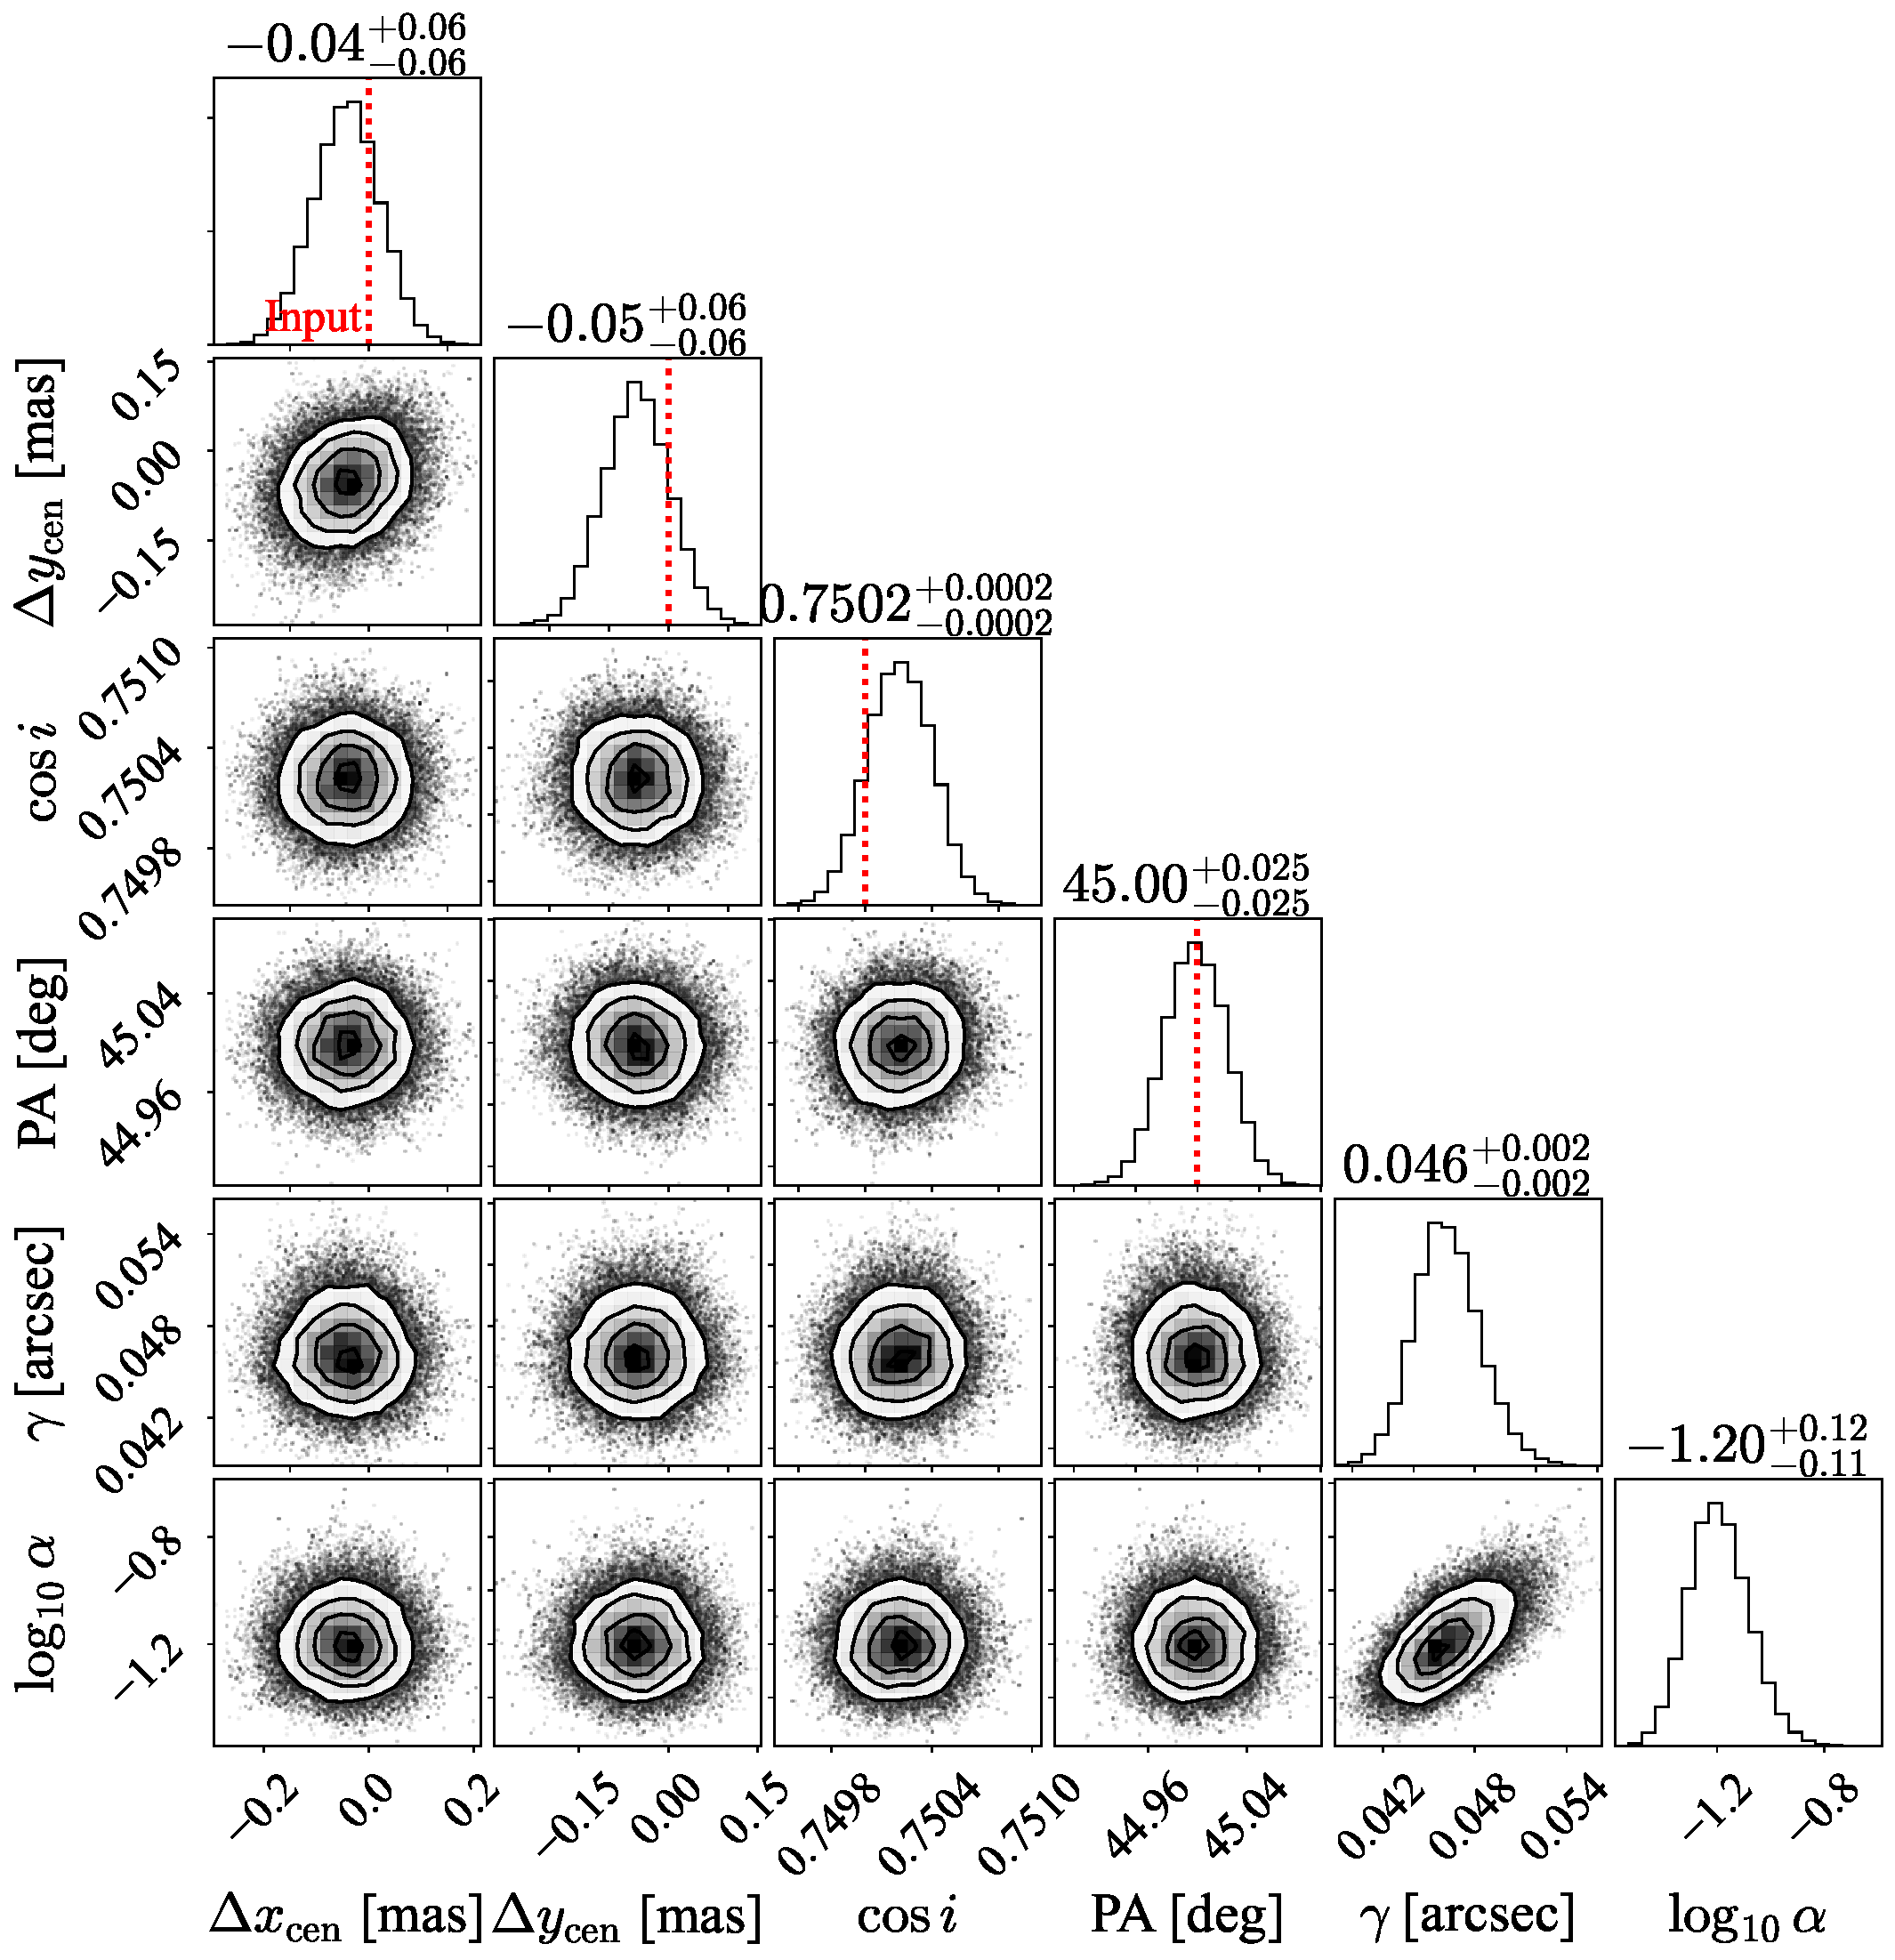
\includegraphics[width=0.48\linewidth]{./fig/recovered_sim_mcmc.pdf}
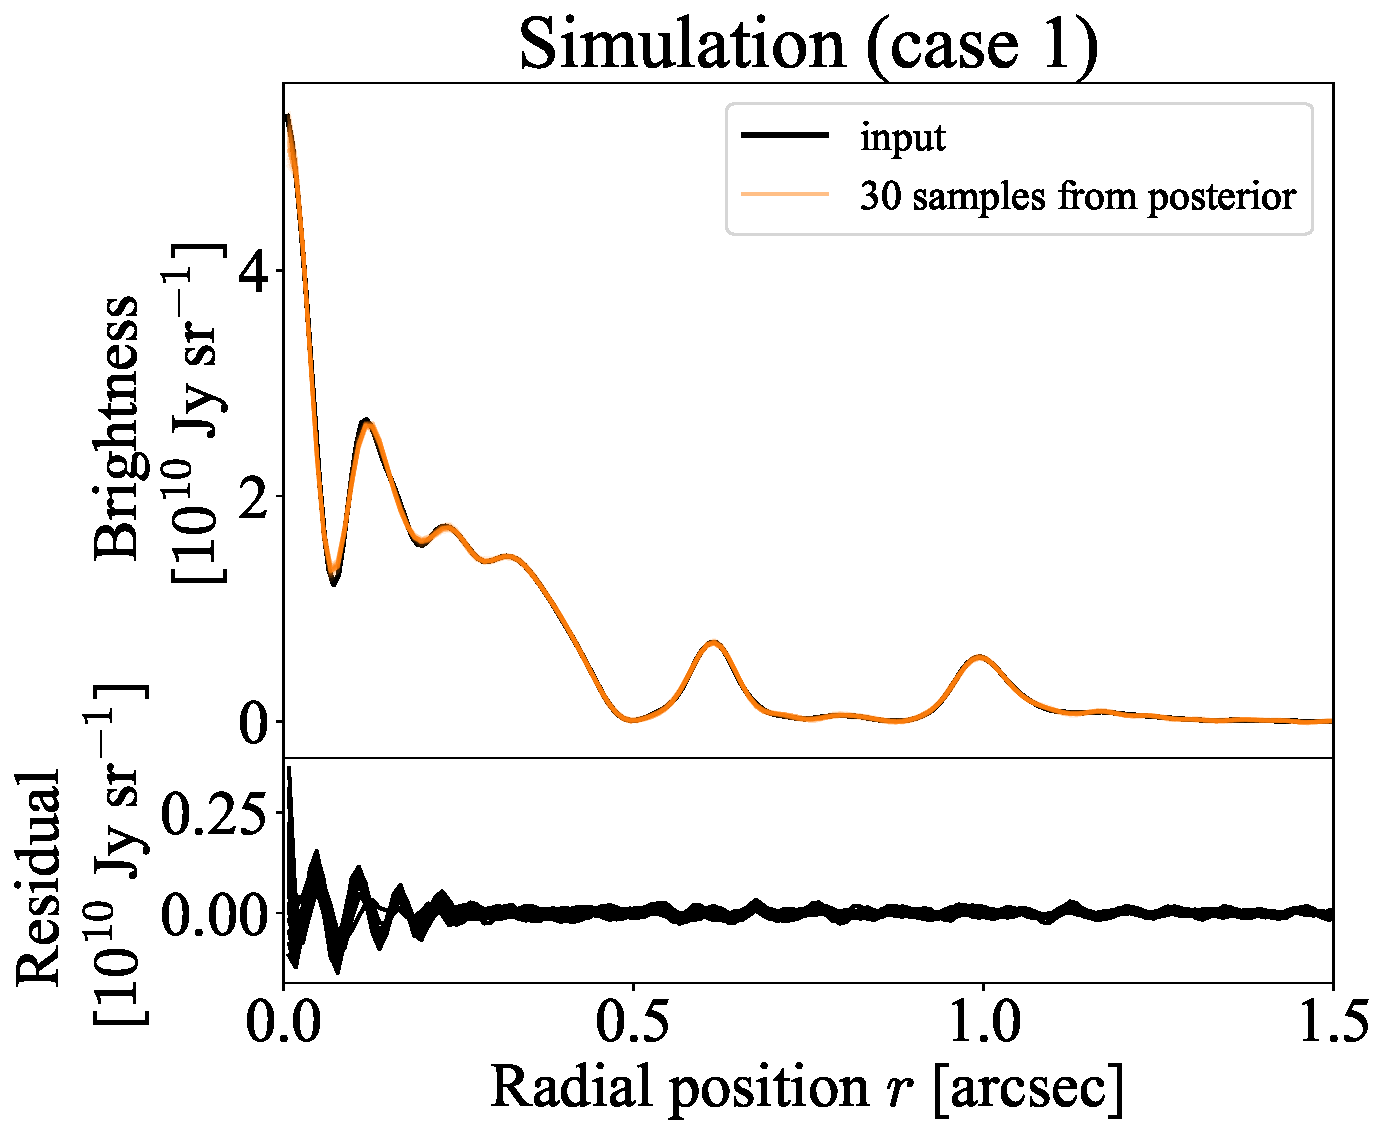
\includegraphics[width=0.48\linewidth]{./fig/posterior_sim.pdf}
\end{center}
\caption{Example for posterior sampling for all of disc parameters. The figure is taken \protect \cite{aizawa2024} (Fig. 2 in the paper)}
\label{fig:posterior_sim}
\end{figure*}
%-----------------------------Figure End------------------------------


\chapter{Install  \label{sec:reuired}}
After downloading the codes, you can install it by typing 
\begin{verbatim}
pip install ./protomidpy
\end{verbatim}
The following  modules are required: 
\begin{itemize}
    \item astropy
    \item emcee
    \item corner
    \item matplotlib
    \item numpy
    \item scipy
    \item pandas
    \item Jupyter notebook
    \item tqdm
\end{itemize}


\chapter{Make configuration files \label{sec:prep_sec}}

\section{Format of input data \label{sec:format_data}}
The data must be in form of ".npz" in numpy, and it needs to contain following items: 
\begin{itemize}
    \item \textbf{u\_obs}: Spatial frequency "u" [lambda]
    \item \textbf{v\_obs}: Spatial frequency "v" [lambda]
    \item \textbf{vis\_obs}: Visibility 
    \item \textbf{wgt\_obs}: Weights 
\end{itemize}
Download test data from \url{https://github.com/2ndmk2/dsharp_averaged_data} for reference. 


\section{Config files}
We have three config files. 
\subsection{MCMC setting (example: \texttt{params/mcmc\_config.dat}) \label{sec:mcmc_config}}
Parameters for emcee and model
\begin{itemize}
    \item \textbf{Nrad} (int) \\
    Number of radial points for model intensity
    \item \textbf{Nbin} (int)\\
    Determine grid size for log-binning. Grid size is (2*Nbin+1, 2*Nbin+1). 
    \item \textbf{Dpix} (float)\\
    Radial spacing for model [arcsec].\\ Outer disk radius is determined as $Rout = Nrad * Dpix$
    \item \textbf{Nwalker}  (int)\\
    Number of walkers for emcee
    \item \textbf{Nchain  (int)}\\
    Number of chains for emcee
    \item \textbf{Qmin}  (float)\\
    Value determining lower boundary for log gridding. 
    \item \textbf{Qmax} (float)\\
    Value determining upper boundary for log gridding. 
    \item \textbf{out\_folder} (str)\\
    Path to output folder
\end{itemize}

\subsection{Initialize positions for walkers (example: \texttt{params/AS209\_paradic.dat})  \label{sec:initial_para}}
Parameters determining initial positions for mcmc. They are randomly generated with uniform distribution [value-scatter/2, value+scatter/2].

\subsection{Prior distribution (example: \texttt{params/prior.dat})  \label{sec:prior_config}}
Parameters for determining ranges of priors: 
\begin{itemize}
    \item {\bf Regularization parameter $\log \alpha$}\\
    Uniform prior, $[\log_{10}\alpha_{\rm min}, \log_{10}\alpha_{\rm max}]$
    \item {\bf Spatial paramter $\gamma$} \\ Uniform prior, [min\_scale [arcsec], max\_scale [arcsec]]
    \item {\bf Central position for disk} \\ 
    Uniform prior,  [-delta\_pos [arcsec], delta\_pos [arcsec]]
\end{itemize}



\chapter{Run scripts \label{sec:run_script}}
\section{Run MCMC (example: \texttt{tests/run\_sampling.py}) \label{sec:mcmc_run}}
\subsection{Overview}

With {\it emcee} \citep{2013PASP..125..306F}, we take samples from posterior distribution for $ p(\bm{g} , \bm{\theta}|\bm{d})$ given as: 
\begin{eqnarray}
   p(\bm{g} , \bm{\theta}|\bm{d}) &\propto&  \mathcal{N}(\bm{d} \mid \bm{0}, \bar{\bm{\Sigma}}_{d} +   \bar{\bm{H}} \bm{\Sigma}_{a} \bar{\bm{H}}^{T}) p(\bm{g} , \bm{\theta}), 
\end{eqnarray}

\subsection{Example command}

\begin{verbatim}
python run_sampling.py --n_process 4 --visfile ./vis_data/
AS209_continuum_averaged.vis.npz --config ./paras/mcmc_config.dat 
--initial_para ./paras/AS209_paradic.dat --prior ./paras/prior.dat 


\end{verbatim}

The options are given as follows: 
    \begin{itemize}
        \item \textbf{n\_process} (int): \\ Number of CPU cores to be used in emcee.
        \item \textbf{visfile} (str): \\ Path to visibility file (\ref{sec:format_data})
        \item \textbf{config } (str):  \\ path to mcmc config file (\ref{sec:mcmc_config}). 
        \item \textbf{initial para} (str): \\ path to mcmc config file (\ref{sec:initial_para}). 
        \item \textbf{prior} (str):  \\ path to mcmc config file (\ref{sec:prior_config}). 
    \end{itemize}

\subsection{Output}
The name for output file is "./result/***\_mcmc.npz". The file includes the following item: 
%

\begin{itemize}
    \item \textbf{sample} (numpy.array, [1, Nwalker*Nchain, 6]): \\ Sample array with size of  taken from posterior distribution. \\ 
    The order for the parameters is 
$(\gamma [{\rm arcsec}], \log_{10} \alpha, \cos {\rm i}, {\rm PA [rad]}, \delta_x{\rm cen}, \delta_y{\rm cen})$.    \item \textbf{log\_prior}: \\ Path to visibility file (\ref{sec:format_data})
    \item \textbf{log\_prior} (numpy.array, [1,Nchain,  Nwalker]): \\ Prior probability. 
    \item \textbf{log\_likelihood} (numpy.array, [1,Nchain,  Nwalker]): \\ Likelihood. 
    \item \textbf{nrad} (int):\\  Number of radial points for model intensity. Same as Nrad.  
    \item \textbf{dpix} (float):\\ Radial spacing for model [arcsec]. Same as Dpix.  
    \item \textbf{n\_bin\_log} (int)::  \\ Determine grid size for log gridding. Same as Nbin. 
    \item \textbf{qmin} (float): \\ Value determining lower boundary for log gridding. 
    \item \textbf{qmax} (float):\\  Value determining upper boundary for log gridding. 
    \item \textbf{cov} (str): Convariance name (default to "RBF"). 
\end{itemize}
    


\section{ Postprocess Calculation  (example: \texttt{tests/model\_calc.py)}}

\subsection{Overview}
Using samples from $p(\bm{g} , \bm{\theta} \mid \bm{d})$, we take sample from full posterior, 
\begin{eqnarray}
  p(\bm{a}, \bm{g} , \bm{\theta} |\bm{d})=p(\bm{a}|\bm{d}, \bm{g} , \bm{\theta}) p(\bm{g} , \bm{\theta} |d), 
\end{eqnarray}
and model visibilities: 
\begin{eqnarray}
\left(\begin{array}{c}
    \bm{V}_{\rm real} \\
    \bm{V}_{\rm imag} 
\end{array}\right)
= 
\left(\begin{array}{cc}
 \bm{C}_{\rm real}\bm{H'} \\
 \bm{C}_{\rm imag}\bm{H'} \\
\end{array}\right)
 \bm{a}, \label{eq:linear_inclined}
\end{eqnarray} 
where $\bm{H'}$, $\bm{C}_{\rm real}$, and $\bm{C}_{\rm imag}$ are defined as follows: 
\begin{eqnarray}
    \{\bm{H'}\}_{j,k} &=&  \displaystyle \frac{4 \pi R_{\rm out}^{2}}{j_{0( N+1)}^{2} J_{1}^{2}(j_{0k})} J_{0} \left(2 \pi q_{j} r_{k} \right),  \\
  \{\bm{C}_{\rm real}\}_{j, k} &=& |\cos i| \cos(-2\pi (\Delta x_{\rm cen} u_{j} + \Delta y_{\rm cen} v_{j})) \delta_{j,k}, \nonumber \\ \\ 
 \{ \bm{C}_{\rm imag}\}_{j, k} &=&  |\cos i| \sin(-2\pi (\Delta x_{\rm cen} u_{j} + \Delta y_{\rm cen} v_{j})) \delta_{j,k}. \nonumber \\ 
\end{eqnarray} 


\subsection{Example command}

\begin{verbatim}
python model_calc.py --n_sample_for_rad 20 --n_burnin 20000
--visfile ./vis_data/AS209_continuum_averaged.vis.npz 
--mcmc_result_file ./result/AS209_continuum_averaged.vis_mcmc.npz
--initial_para ./paras/AS209_paradic.dat --prior ./paras/prior.dat 
--out_file_for_model ./result/AS209_continuum_averagedmodel.npz
\end{verbatim}

The options are given as follows: 

\begin{itemize}
    \item \textbf{n\_sample\_for\_rad} (int): Number of samples for intensity profiles
    \item \textbf{n\_burnin} (int): Number of Burnin samples
    \item \textbf{visfile} (str): Path to visibility file (\ref{sec:format_data})
    \item \textbf{mcmc\_result\_file (str)}: Path to result file from \texttt{run\_sampling.py} (\ref{sec:mcmc_run})
    \item \textbf{out\_file\_for\_model} (str): Path to output file 
\end{itemize}


\subsection{Output}
The name for output file is "./result/***model.npz". The file includes the following item: 


\begin{itemize}
    \item \textbf{r\_n}  (numpy.array, [Nrad]): \\ 
    Radial positions  [arcsec] for model intensities 
    \item \textbf{param\_map} (numpy.array, [6]): \\ 
    MAP solution for parameters.
    \item \textbf{params\_random\_selected} (numpy.array, [n\_sample\_for\_rad, 6]): \\ 
    Randomly selected parameters with size of n\_sample\_for\_rad.
    \item \textbf{flux\_map\_sample} (numpy.array, [200]): \\ 
    Model intensity $\bm{a}^{\dagger}$  [Jy arcsec$^{-2}$]  taken from posterior assuming Maximum a posteriori estimation (MAP) solution for non-linear parameters $\bm{g}_{\rm MAP}, \bm{\theta}_{\rm MAP}$, which are taken from the result of MCMC. 
    \item \textbf{flux\_random\_samples} (numpy.array, [n\_sample\_for\_rad, Nrad]): \\ 
    Randomly selected model intensities [Jy arcsec$^{-2}$] with size of n\_sample\_for\_rad.
    \item \textbf{vis\_model\_undeprojected} (numpy.array, [Nvis]): \\ 
    Undeprojected visibility models [Jy] with size of Nvis assuming $(\bm{a}^{\dagger}, \bm{g}_{\rm MAP}, \bm{\theta}_{\rm MAP})$.
    \item \textbf{residual\_undeprojected} (numpy.array, [Nvis]): \\ 
    Undeprojected residual visibilties  [Jy] with size of Nvis   assuming $(\bm{a}^{\dagger}, \bm{g}_{\rm MAP}, \bm{\theta}_{\rm MAP})$.
    \item \textbf{qdist\_deprojected} (numpy.array, [Nvis]): \\ 
    Deprojected spatial frequency distance $q$ [lambda] with size of Nvis  assuming $(\bm{a}^{\dagger}, \bm{g}_{\rm MAP}, \bm{\theta}_{\rm MAP})$
    \item \textbf{vis\_model\_deprojected} (numpy.array, [Nvis]): \\ 
    Deprojected visibility models [Jy] with size of Nvis  assuming $(\bm{a}^{\dagger}, \bm{g}_{\rm MAP}, \bm{\theta}_{\rm MAP})$. 
    \item \textbf{data\_deprojected} (numpy.array, [Nvis]): \\ 
    Deprojected data  [Jy] with size of Nvis assuming $(\bm{a}^{\dagger}, \bm{g}_{\rm MAP}, \bm{\theta}_{\rm MAP})$. 
    \item \textbf{data\_weights} (numpy.array, [Nvis]): \\ 
    Weights  [Jy$^{-2}$] for the deprojected data with size of Nvis  assuming $(\bm{a}^{\dagger}, \bm{g}_{\rm MAP}, \bm{\theta}_{\rm MAP})$. 
\end{itemize}
    
\section{See result (example: \texttt{tests/mcmc\_plotter.ipynb})}
Run \texttt{mcmc\_plotter.ipynb} with Jupyter. We use following variables to specity files to be loaded. 
    \begin{itemize}
        \item \textbf{samplefile}: Path to file for posterior sampling output from \texttt{run\_sampling.py}
        \item \textbf{modelfile}: Path to postprocess result from \texttt{model\_calc.py}
    \end{itemize}

\bibliography{ref.bib}

\end{document}